Section \ref{subsec:consensusArchetypes} explains that six consensus archetypes are found to emerge across seven datasetets. In the following the methods used to arrive at this result is explained.

Employing archetypal analysis on a for a large number of points prove problematic when the domain is constrained (in this case from [-1 ; 1]), because noise in the data causes all subdomains of the space to fill up. For BF datapoints which exist in five dimensions, the full dataset therefore constitute a 5D cube (a \textti{hypercube}), which leads the archetypes to snap the the vertices of this box. Therefore a different approach is taken. Considering Figure \ref{fig:convexHullCurseOfDimensionality} the convex hull in five dimensions of just 200 points only contains about 20\% of the datapoints in a point cloud. Furthermore, 200 points are found to constitute a small enough subset that points rarely go to the geometrical extremes of the domain. Howver, it is observed that using such a small number of points often leads to archetypes that are very different between iterations, and as such the following approach for finding the archetypes is taken (all references to row sorting use the algorithm shown in Python code in Listing \ref{lst:reorder_to}):

\begin{enumerate}
	\item Compute archetype 5000 times for subsets of 200 points for each of the seven datasets, using Python implementation of AA\mcite{pypcha}. This yields a tensor $\matr{X}$ which has dimensions $(N=6) \times (M=5) \times (K=5000)$, where $N$ are archetypes, $M$ are BFTs and $K$ are iteration slices, indexed $i$, $j$, $k$, respectively (see Figure \ref{fig:entryWiseStatistics}).
	\item For each dataset:
	\begin{enumerate}
		\item For each pair of iteration slices (of which there are $(K-1)^2/2$) sort rows to minimize average distance between points, and record the distance between the pairs. Remove the 50\% of all iteration slices starting with the ones of highest average distance to other slices.
		\item In two-iteration steps, sort rows of $\matr{X}_{k+1}$ with respect to rows of $\matr{X}_{k}$ such as to minimize average distance between archetypes. Replace pair with average along 2nd axis. Repeat until there is only one slice left. This constitutes the archetypes of the dataset.
	\end{enumerate} 
	\item Sort resulting rows for each dataset using one as a reference. This yields the archetypes shown in Figure \ref{fig:medianDistances}. Stack them in depth to form a matrix of shape $6 \times 5 \times 7$ and compute the SD and median matrices along the 2nd axis, $\matr{\Sigma}$ and $\matr{A}$ respectively.
	\item Repeat step (3) 1000 times where columns in each slice are shuffled, and record the distribution of SDs along the 2nd axis. Take the maximum value of the 5th percentile as a threshold, $\lambda$, for maximally allowed SD between archetype traits (consensus threshold, see Figure \ref{fig:varianceThreshold}).
	\item Enforce $\lambda$ on $\matr{\Sigma}$ and apply the resulting mask to $\matr{A}$ to reveal the consensus archetypes.
\end{enumerate}

\begin{figure}
	\centering
	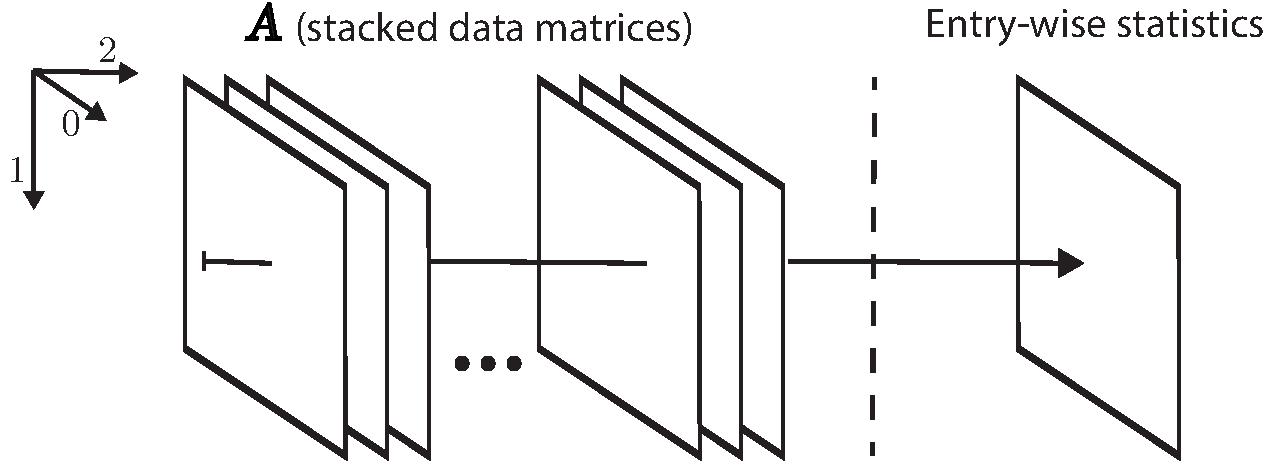
\includegraphics[width=1\textwidth]{figures/entryWiseStatistics}
	\caption{\label{fig:entryWiseStatistics} Example of how 2D matrices are stacked to shape a 3D tensor. The coordinate system explains the use of axis labels in the text, and the 'Entry-wise statistics' matrix illustrates how e.g. SD, mean or median values result from computing such along the 2nd axis.}
\end{figure}

% python code
\definecolor{codegreen}{rgb}{0,0.6,0}
\definecolor{codegray}{rgb}{0.5,0.5,0.5}
\definecolor{codepurple}{rgb}{0.58,0,0.82}
\definecolor{backcolour}{rgb}{0.95,0.95,0.92}
 
\lstdefinestyle{mystyle}{
    backgroundcolor=\color{backcolour},   
    commentstyle=\color{codegreen},
    keywordstyle=\color{magenta},
    numberstyle=\tiny\color{codegray},
    stringstyle=\color{codepurple},
    basicstyle=\footnotesize,
    breakatwhitespace=false,         
    breaklines=true,                 
    captionpos=b,                    
    keepspaces=true,                 
    numbers=left,                    
    numbersep=5pt,                  
    showspaces=false,                
    showstringspaces=false,
    showtabs=false,                  
    tabsize=2
}
 
\lstset{style=mystyle}

\begin{lstlisting}[language=Python, label={lst:reorder_to}, caption="Python code for sorting rows of matrix $\matr{A}$ to match those of $\matr{B}$"]
import numpy as np
def reorder_to(A, B):
    """Return order of rows in A the best match rows in B."""
    distance_matrix = np.ones((6, 6))*np.inf
    for i, a in enumerate(A):
        for ii, b in enumerate(B):
            ba = (b-a)
            distance_matrix[i, ii] = np.sqrt(np.dot(ba, ba))
    reorder = [[] for _ in range(6)]
    for _ in range(6):
        ind = np.argmin(distance_matrix)
        i, ii = ind/6, ind%6
        reorder[ii] = i
        distance_matrix[i, :] = np.inf
        distance_matrix[:, ii] = np.inf
    return reorder
\end{lstlisting}